\section{三角不等式的证明}
\label{sec:proof-spectral-triangle-inequality}

证明三角不等式之前，须先回忆裤子乘积
\[
 HF_*(H_1,J^1)\otimes HF_*(H_2,J^2)\longrightarrow HF_*(H_3,J^3)
\]
的定义。为研究乘积对滤过的影响，需要像 (Oh99)、(Schw00) 那样在链层以最优方式
定义此乘积。

弗洛尔同调裤子乘积的链层结构常数，由在穿孔附近插值如下弗洛尔方程的扰动伪全纯
方程之刚性解的“数目”给出：
\[
 \frac{\partial u}{\partial\tau}
 +J_i\left(\frac{\partial u}{\partial t}-X_{H_i}(u)\right)=0,
 \qquad i=1,2,3.
\]
弗洛尔方程特别使用定义域 $\mathbb R\times\mathbb R/\mathbb Z$ 的圆柱结构与坐标
$(\tau,t)$，而一般黎曼曲面 $S$ 没有全局坐标，因此构造中须使用其不变形式
\[
 (du+P_K(u))_J^{(0,1)}=0.
\]
证明三角不等式时，相关哈密顿量三元组 $(H_1,H_2;H_3)$ 必须满足相应共轭类关系
\[
 [\phi_{H_1}]^{-1}[\phi_{H_2}]^{-1}[\phi_{H_3}]=\mathrm{id}.
\]
例如可取 $H_3=H_1\#H_2$；注意三元组
$(\overline H_1,\overline H_2,H_1\#H_2)$ 在 4.3.1 节定义的和乐类平凡。

以下引理是研究谱不变量三角不等式的关键。这里把
$\operatorname{curv}(\Gamma)$ 或 $R_K$ 看作由 $\dot\Sigma$ 参数化的哈密顿量族。

\begin{definition}
\label{def:21-hofer-norm-family}
设 $K\in C^\infty(\dot\Sigma,C_0^\infty(M))$。定义 $K$ 的 $L^\infty$ 霍费尔范数为
\begin{equation}
 \lVert K\rVert_\infty:=\sup_{z\in\dot\Sigma}\operatorname{osc}K_z
 =\sup_{z\in\dot\Sigma}(\max K_z-\min K_z),
 \label{eq:21-linfty-hofer-family}
\end{equation}
并定义 $L^{(1,\infty)}$ 霍费尔范数为
\begin{equation}
 \lVert K\rVert_{1,\infty}:=
 \int_{\dot\Sigma}\operatorname{osc}K_z\,dA_\Sigma
 =\int_{\dot\Sigma}(\max K_z-\min K_z)\,dA_\Sigma.
 \label{eq:21-loneinfty-hofer-family}
\end{equation}
\end{definition}

\begin{lemma}
\label{lem:21-small-curvature-connection}
设 $H_i$ 是满足 $H_1\#H_2=H_3$ 的三元组，并考虑和乐
$(\overline H_1,\overline H_2,H_1\#H_2)$。对任意 $\delta>0$，可选取和乐类为
\[
 C=([\phi_{H_1}^{-1}],[\phi_{H_2}^{-1}],[\phi_{H_1}\phi_{H_2}])
\]
的哈密顿联络 $\Gamma$，使其曲率范数满足
\[
 \lVert\operatorname{curv}(\Gamma)\rVert_\infty
 =\lVert R_K\rVert_\infty\leq\delta.
\]
\end{lemma}

\begin{proof}
\stfhIndex{I130}{Jixiaomianjiduliang}{极小面积度量（minimal area metric）}
先回忆如何利用\emph{极小面积度量} (Z93) 描述亏格 $0$、带三个穿孔的紧黎曼曲面
$\Sigma$ 的共形结构。将 $\Sigma$ 共形地视为三个半圆柱 $\Sigma_1,\Sigma_2,\Sigma_3$
之并，每个半圆柱配备平坦度量，其子午圆周长为 $2\pi$。度量只在位于
$\Sigma_i$ 边界圆周上的两点 $p,\bar p\in\Sigma$ 处奇异，因此度量诱导的共形结构
自然延拓越过 $p,\bar p$。所得结构正是
$\Sigma=S^2\setminus\{z_1,z_2,z_3\}$ 上唯一的标准共形结构。该\emph{奇异}度量除
$p,\bar p$ 外处处平坦；在这两点虽奇异却是利普希茨的。它是所谓极小面积度量的
例子。茨维巴赫 (Z93) 在弦场论中构造\emph{弦顶点}时曾广泛研究这种度量；见图
\ref{fig:21-minimal-area-metric}。

\begin{figure}[htbp]
 \centering
 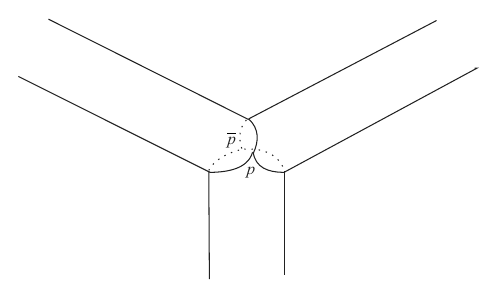
\includegraphics[width=.52\textwidth]{chapters/ch21-spectral-construction/figures/figure-21-1.png}
 \caption{一个极小面积度量。}
 \label{fig:21-minimal-area-metric}
\end{figure}

按如下方式把 $\Sigma$ 认作 $\Sigma_i$ 之并：
\[
 \Sigma=\bigcup_{i=1}^3\Sigma_i.
\]
若把 $\Sigma_i$ 等同于 $(-\infty,0]\times S^1$，则 $\Sigma$ 中存在三条从 $p$ 连接
到 $\bar p$、长度为 $1/2$ 的道路 $\theta_i$，$i=1,2,3$，使
\begin{equation}
 \begin{aligned}
 \partial_1\Sigma&=\theta_1\circ\theta_3^{-1},\\
 \partial_2\Sigma&=\theta_2\circ\theta_1^{-1},\\
 \partial_3\Sigma&=\theta_3\circ\theta_2^{-1}
 =(\theta_1\circ\theta_3^{-1})^{-1}\circ
 (\theta_2\circ\theta_1^{-1})^{-1}.
 \end{aligned}
 \label{eq:21-pants-gluing-rule}
\end{equation}
在这些坐标中，$p,\bar p$ 分别对应 $(s,t)=(0,0),(0,1/2)$。对 $i=1,2$ 固定
$\Sigma_i$ 与 $(-\infty,0]\times S^1$ 的全纯等同，其中
$S^1=\mathbb R/2\pi\mathbb Z$；并据分解~\eqref{eq:21-pants-gluing-rule} 把
$\Sigma_3$ 等同于 $[0,\infty)\times S^1$。记这些等同为
\[
 \varphi_i^-:\Sigma_i\to(-\infty,0]\times S^1,\quad i=1,2,
 \qquad
 \varphi_3^+:\Sigma_3\to[0,\infty)\times S^1,
\]
前者对应正穿孔，后者对应负穿孔；圆柱上的标准坐标记为 $(\tau,t)$。

现于三份 $[0,1]^2$ 上构造显式的哈密顿微分同胚二参数族。用
\eqref{eq:21-reparameterization-cutoff} 型函数对同痕的时间 $t$ 重参数化后，可设
$\phi_i$ 在 $t=0,1$ 附近关于时间为常值。公式为
\[
 \phi_1(s,t)=
 \begin{cases}
 \phi_{H_1}^{(1-s)t/(1-s/2)},&0\leq t\leq1-s/2,\\
 \phi_{H_1}^{1-s}\phi_{H_2}^{2(t-1+s/2)/s},&1-s/2\leq t\leq1,
 \end{cases}
\]
\[
 \phi_2(s,t)=
 \begin{cases}
 \phi_{H_1}^{2t},&0\leq t\leq s/2,\\
 \phi_{H_1}^{s}\phi_{H_2}^{(t-s/2)/(1-s/2)},&s/2\leq t\leq1,
 \end{cases}
\]
以及
\[
 \phi_3(s,t)=
 \begin{cases}
 \phi_{H_1}^{t(1+s)}\phi_{H_2}^{t(1-s)},&0\leq t\leq1-s/2,\\
 \phi_{H_1}^{(1+s)(1-s/2)}
 \phi_{H_2}^{2(t-1+s/2)/s},&1-s/2\leq t\leq1.
 \end{cases}
\]

\begin{exercise}
\label{ex:21-pants-family-compatibility}
核验该族与粘合规则~\eqref{eq:21-pants-gluing-rule} 的相容性，以及它在
$p,\bar p$ 之外的光滑性。
\end{exercise}

此外，从公式也可看出
\[
 \phi_1(0,t)=\phi_{H_1}^t,\qquad
 \phi_2(0,t)=\phi_{H_2}^t,\qquad
 \phi_3(1,t)=\phi_{H_1}^t\phi_{H_2}^t.
\]
相应联络在 $p,\bar p$ 外的平坦性，显然来自上述光滑的哈密顿微分同胚二参数族。

再用\termElongationFunction{}~$\rho$ 沿 $s$ 方向拉长裤子，得到 $\Sigma$ 上除 $p,\bar p$ 外处处光滑
的平坦联络。记平凡丛 $\dot\Sigma\times M\to\dot\Sigma$ 上的联络 1-形式为
\footnote{译者注：原文把联络 1-形式 $K$ 排成从 $\dot\Sigma$ 到
$\Omega^1(\dot\Sigma,C_0^\infty(M))$ 的映射，类型上似乎多出一层 $\dot\Sigma$；
译文照录。}
\[
 K:\dot\Sigma\longrightarrow\Omega^1(\dot\Sigma,C_0^\infty(M)).
\]
由于 $H_1,H_2$ 在边界附近平坦，它也在 $p,\bar p$ 处光滑，且曲率为 $0$。
\end{proof}

\begin{remark}
\label{rem:21-concatenation-hamiltonian}
同伦类 $[H_1\#H_2]$ 还可由拼接哈密顿量
\[
 H_1*H_2(t,x)=
 \begin{cases}
 2H_1(2t,x),&t\leq1/2,\\
 2H_2(2t-1,x),&t\geq1/2
 \end{cases}
\]
实现，而不必用 $H_1\#H_2$。这里假设 $H_1,H_2$ 在 $t=0,1$ 附近均边界平坦，
以保证相应联络光滑。这给出三元组 $(H_1,H_2;H_1*H_2)$ 所伴随的稍有不同的哈密顿
纤维化。不过 $H_1\#H_2$ 与 $H_1*H_2$ 同伦，故可把后者作为第三个哈密顿量
$H_3$；此时平坦联络的构造比使用 $H_1\#H_2$ 更明显。只须取
$\phi_3(s,t)\equiv\phi_3(0,t)$，并注意
\[
 \phi_3(0,t)=
 \begin{cases}
 \phi_{H_1}^{2t},&0\leq t\leq1/2,\\
 \phi_{H_1}^1\phi_{H_2}^{2t-1},&1/2\leq t\leq1,
 \end{cases}
\]
这正是道路 $\phi_{H_1}*\phi_{H_2}:t\mapsto\phi_{H_1*H_2}^t$。事实上，上述
$\phi_3$ 公式给出 $\phi_{H_1*H_2}$ 与 $\phi_{H_1}\phi_{H_2}$ 之间的显式同伦。
更多细节见 (FOOO11b)。
\end{remark}

现在证明三角不等式。令 $\alpha\in CF_*(H)$、$\beta\in CF_*(F)$ 是满足
$[\alpha]=a^\flat,[\beta]=b^\flat$ 的弗洛尔闭链，并令其裤子乘积闭链
$\alpha*\beta=:\gamma\in CF_*(H\#F)$。则
$[\alpha*\beta]=(a\cdot b)^\flat$，所以
\begin{equation}
 \rho(H\#F;a\cdot b)\leq\lambda_{H\#F}(\alpha*\beta).
 \label{eq:21-triangle-product-level}
\end{equation}
给定 $\delta>0$，选取 $\alpha,\beta$ 使
\begin{align}
 \lambda_H(\alpha)&\leq\rho(H;a)+\delta/2,
 \label{eq:21-alpha-near-minimax}\\
 \lambda_F(\beta)&\leq\rho(F;b)+\delta/2.
 \label{eq:21-beta-near-minimax}
\end{align}
于是可写
\[
 \alpha=\sum_i a_i[z_i,w_i],\quad
 \mathcal A_H([z_i,w_i])\leq\rho(H;a)+\delta/2,
\]
\[
 \beta=\sum_j a_j[z_j,w_j],\quad
 \mathcal A_F([z_j,w_j])\leq\rho(F;b)+\delta/2.
\]
下面用裤子乘积 (20.2.29) 估计 $\alpha*\beta\in CF_*(H\#F)$ 的层级。

回忆 (4.3.16) 与命题~\ref{prop:20-energy-curvature-identity} 中的恒等式
\[
 \int v^*\Omega_E=-\mathcal A_{H_1\#H_2}([z_3,w_3])
 +\mathcal A_{H_1}([z_1,w_1])+\mathcal A_{H_2}([z_2,w_2])
\]
及
\[
 E_{(K,J)}(u)=\int v^*\Omega_E+R_K(u),
\]
其中对任意 $u\in\mathcal M(K,J;\widetilde z)$，$v(z)=(z,u(z))$。
按 $*$ 的定义，对任意 $[z_3,w_3]\in\alpha*\beta$，存在
$[z_1,w_1]\in\alpha$、$[z_2,w_2]\in\beta$，使
$\mathcal M(K,J;\widetilde z)$ 在渐近条件
\[
 \widetilde z=([z_1,w_1],[z_2,w_2];[z_3,w_3])
\]
下非空。应用引理~\ref{lem:21-small-curvature-connection} 及
\eqref{eq:21-triangle-product-level}--\eqref{eq:21-beta-near-minimax}，立即得到
\begin{align}
 \mathcal A_{H\#F}([z_3,w_3])
 &\leq\mathcal A_H([z_1,w_1])+\mathcal A_F([z_2,w_2])+\delta\notag\\
 &\leq\lambda_H(\alpha)+\lambda_F(\beta)+\delta\notag\\
 &\leq\rho(H;a)+\rho(F;b)+2\delta
 \label{eq:21-triangle-action-estimate}
\end{align}
对所有 $[z_3,w_3]\in\alpha*\beta$ 成立。合并
\eqref{eq:21-triangle-product-level}--\eqref{eq:21-triangle-action-estimate}，有
\[
 \rho(H\#F;a\cdot b)\leq\rho(H;a)+\rho(F;b)+2\delta.
\]
令 $\delta\to0$，即得
\[
 \rho(H\#F;a\cdot b)\leq\rho(H;a)+\rho(F;b),
\]
三角不等式得证。
